% Source: 2006湖北文.pdf, source-relative PDF page 1, Q18.
% Non-scale vector redraw; solid/dashed visibility follows the fixed candidate image.
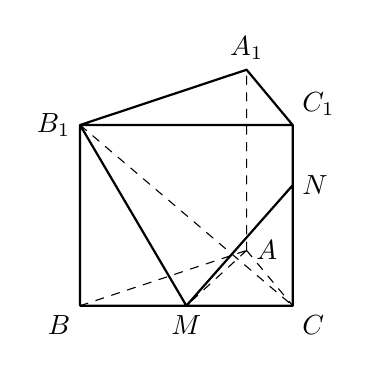
\begin{tikzpicture}[line cap=round,line join=round,x=0.9cm,y=0.9cm]
  \coordinate (B)  at (0,0);
  \coordinate (C)  at (3,0);
  \coordinate (M)  at (1.5,0);
  \coordinate (A)  at (2.35,0.78);
  \coordinate (B1) at (0,2.55);
  \coordinate (C1) at (3,2.55);
  \coordinate (N)  at (3,1.70);
  \coordinate (A1) at (2.35,3.33);

  % Hidden/inner lines visible dashed in the source drawing.
  \draw[dashed] (B)--(A) (A)--(C) (A)--(A1) (B1)--(C) (A)--(M);

  % Prism edges and the two solid segments through M shown in the source.
  \draw[thick] (B)--(C) (B)--(B1) (B1)--(C1) (C)--(C1)
    (B1)--(A1)--(C1) (B1)--(M) (M)--(N);

  \node[below left] at (B) {$B$};
  \node[below] at (M) {$M$};
  \node[below right] at (C) {$C$};
  \node[left] at (B1) {$B_1$};
  \node[above] at (A1) {$A_1$};
  \node[above right] at (C1) {$C_1$};
  \node[right] at (N) {$N$};
  \node[right] at (A) {$A$};
\end{tikzpicture}
